
\hypertarget{contas-puxfablicas-estadual}{%
\chapter{Contas Públicas Estadual}\label{contas-puxfablicas-estadual}}

O resultado primário do Estado no acumulado até o quarto bimestre de
2020 foi de cerca de R\$ 1,08 bilhões, valor 73\% maior que o resultado
primário acumulado no mesmo período de 2019, quando foi pouco mais de
R\$ 622 milhões. No primeiro bimestre de 2020 a receita primária foi
30\% maior quando comparado com o primeiro bimestre de 2019. O resultado
primário representa o esforço fiscal do governo para diminuir o estoque
da dívida. A figura \ref{fig:var_receita_despesa_primaria} apresenta
variação da receita e despesa primária acumulada até o bimestre em
relação ao mesmo período do ano passado.

No quarto bimestre a receita primária apresentou um crescimento de 10\%
no acumulado até quarto bimestre, representando um desempenho melhor que
2019, quando a crescimento da receita primária foi de pouco menos de
10\%. As despesas primária cresceu somente 2,03\%, no mesmo período de
2019 cresceu 6,48\%. O baixo crescimento da despesas primária em 2020
contribuiu para um resultado primário elevado até o quarto bimestre de
2020.

Observando as despesas por categoria -- figura \ref{fig:var_despesa_categoria} --
no acumulado até o quarto bimestre houve aumento nos gastos com assistência
social, que cresceram 132\% em
relação ao quarto bimestre de 2019. Gastos da previdência social também
apresentou crescimento na ordem de 16,25\%, seguido pelos gastos com
saúde crescendo 12,85\% em relação a 2019.

Gastos com administração, educação e segurança pública encolheu -6,85\%,
-5,69\% e -12,69\% respectivamente.

\begin{figure}[!h]
	\begin{subfigure}{\linewidth}
		\caption{\label{fig:var_receita_despesa_primaria}Variação da receita e despesa primária acumulada}
		\subcap{Variação acumulada em relação ao bimestre do ano anterior}
		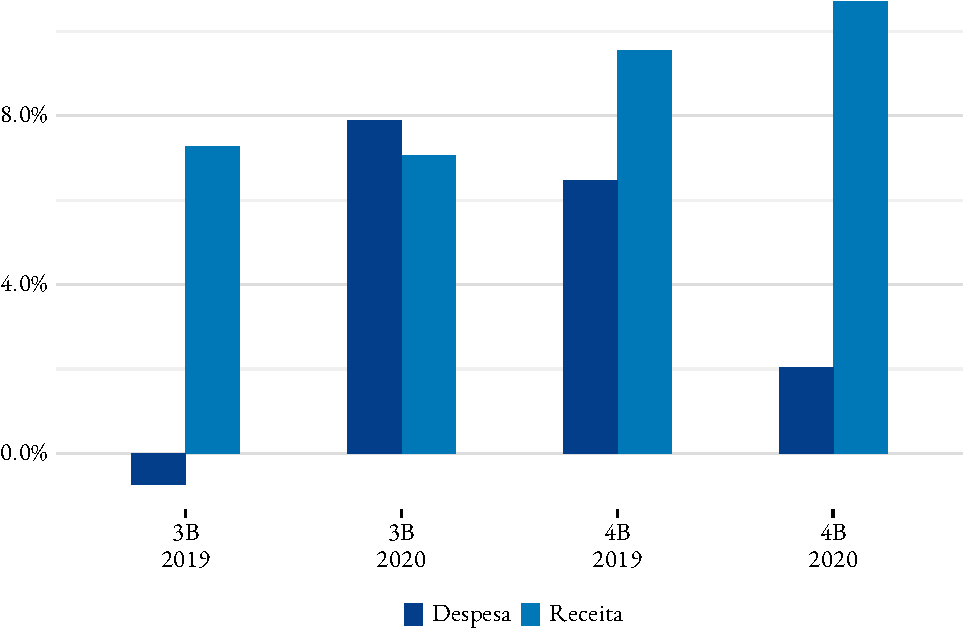
\includegraphics{fig/var_receita_despesa_primaria-1.pdf}
		\source{\acrshort{siconfi}/Tesouro Nacional}
	\end{subfigure}
	\begin{subfigure}{\linewidth}
		\caption{\label{fig:var_despesa_categoria}Variação da despesa por categoria}
		\subcap{Variação acumulada em relação ao bimestre do ano anterior}
		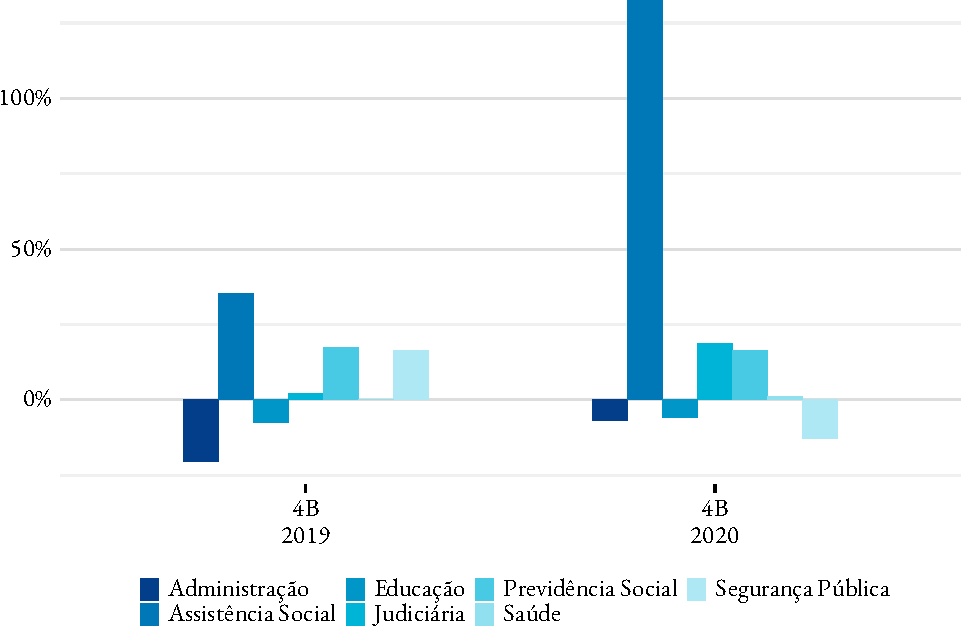
\includegraphics{fig/var_despesa_categoria-1.pdf}
		\source{\acrshort{siconfi}/Tesouro Nacional}
	\end{subfigure}
	\begin{subfigure}{\linewidth}
		\caption{\label{fig:desp_pessoal_rcl}Despesa Total com Pessoal em relação à RCL}
		\subcap{RCL e despesa acumulada até agosto}
		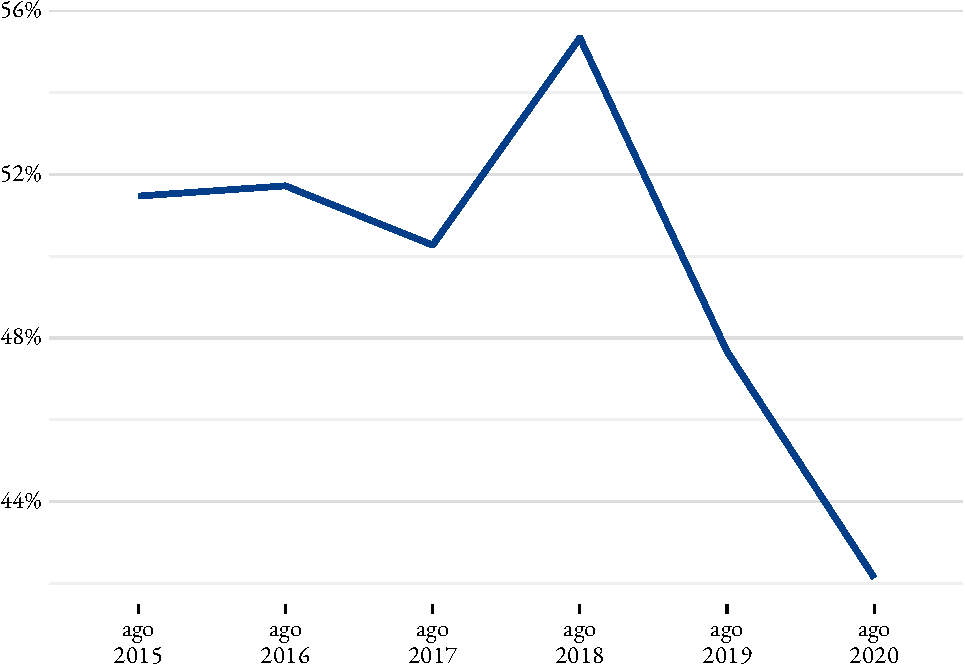
\includegraphics{fig/desp_pessoal_rcl-1.pdf}
		\source{\acrshort{siconfi}/Tesouro Nacional}
	\end{subfigure}
\end{figure}

As despesas com pessoal em relação a receita corrente líquida
\acrshort{rcl}, figura \ref{fig:desp_pessoal_rcl}, mostra parcela da
\acrshort{rcl} destinada ao pagamento de despesas com pessoal no
acumulado do quarto bimestre de cada ano. Até agosto as despesas com
pessoal em relação a \acrshort{rcl} diminui pelo segundo ano seguido. No
segundo quadrimestre de 2015 essa relação estava em 51,5\%, acima do
limite máximo de 49\% para o executivo estabelecido na \acrshort{lrf}.
Em 2016 ficou em 51,7\%, seguido por uma leve reducação em 2017, em 2018
as despesas em proporção a \acrshort{rcl} chegou em 55,3\%. De 2019 a
2020 a redução na relação foi de -11,74\%.

A dívida consolidada líquida (\acrshort{dcl}) do Estado em relação a
\acrshort{rcl} até agosto apresentou queda. Em agosto de 2020 a relação
\acrshort{dcl}/\acrshort{rcl} ficou em 44,1\%, valor abaixo do limite
definido pelo Senado Federal para os Estados, de duas vezes a receita
corrente líquida. Entre 2017 e 2017 a \acrshort{dcl} em proporção à
\acrshort{rcl} aumentou, saindo de 30\% para 52,3\% em 2019 -- figura
\ref{fig:divida_rcl}.

\begin{figure}[!h]
	\begin{subfigure}{\linewidth}
		\caption{\label{fig:}Dívida Consolidada Líquida em relação à RCL}
		\subcap{RCL e DCL acumulada até agosto}
		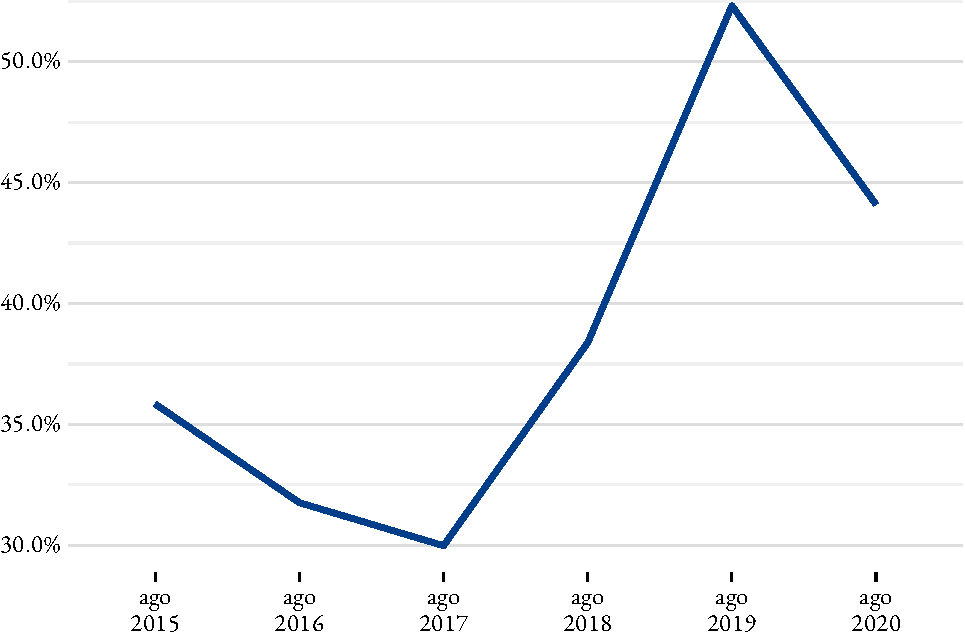
\includegraphics{fig/divida_rcl-1.pdf}
		\source{\acrshort{siconfi}/Tesouro Nacional}
	\end{subfigure}
\end{figure}

O capacidade de pagamento (\acrshort{capag}) traz informações a cerca da
situação fiscal do Estados e Munícipois. A nota é utlizada para Estados
contrair empréstimos com garantia do Governo Federal. A nota atribuida a
cada Estado (A, B ou C) ou Município é derivada de três indicadores:
endividamento, poupança corrente e liquidez. Em 2020 apenas o Espírito
Santo obteve nota A. O Tocantins ficou com nota C por três anos
seguidos -- tabela \ref{tab:capag}. Notas A e B permite que o Estado receba garantia da União para
solicitar novos empréstimos.

Dos Estados da região norte, os que apresentaram pior nota foi Roraima e
Tocantins. Rondônia aparece como o Estado com melhor evolução, Saiu de B
para A entre 2019-2020, a queda no endividamento de 65,41\% para 57,6\%
e a redução na relação obrigações financeiras/disponibilidade de caixa e
a queda na sua liquidez para 19,1\% garantiu nota A em todos os
indicadores.

O Tocantins apesar de manter a mesma nota, teve pioras em todos os
indicadores: endividamento, poupança corrente e liquidez. O
endividamento que representa a dívida consolidada bruta em relação a
receita corrente líquida aumentou de 46,35\% para 67,6\%, a poupança
corrente que corresponde a relação despesas correntes e receita
correntes ajustadas também apresentou uma pequena piora, aumentou de
94,56\% para 95,9\%. Um índice de poupança corrente menor garante nota
maior, pois melhor será a capacidade da receita corrente de financiar
investimentos. O último indicador, liquidez, foi de 577,5\% em 2020,
ante 539,40\% em 2019.

para obter nota A, o Estado ou Município deve ter um índice menor que
100\%, o que significa que sua disponibilidade em caixa é maior que suas
obrigações financeiras. O Tocantins tem um índice de 577,5\%, em 2019
era 539,40\%.

De todos os indicadores do Estado, endividamento e poupança corrente
estão em melhor situação, pois estão mais próximo do limite para receber
uma melhor nota. Para conseguir uma nota A no índice de endividamento o
Estado deve conservá-lo abaixo de 60\%, atualmente está com 67,6\%. No
índice de poupança corrente, para garantir uma nota B o índice deve
maior ou igual a 90\% e menor que 95\%. Para uma nota A, basta que seja
menor que 90\%, atualmente está em 95,9\%, bem próximo de 95\%. O índice
de liquidez é uma situação mais delicada para o Estado, ele tem maior
peso na nota final. Para obter uma nota B é necessário obter A no índice
de liquidez e nota acima de C (B ou A) na poupança, independente da nota
do endividamento.

\begin{table}[!h]
\caption{\label{tab:capag}Nota da capacidade de pagamento}
	\subcap{Indicadores da CAPAG}
\begin{tabu} to \linewidth {>{\raggedright}X>{\centering}X>{\centering}X>{\centering}X>{\centering}X>{\centering}X>{\centering}X}
\toprule
\multicolumn{1}{c}{ } & \multicolumn{2}{c}{Endividamento} & \multicolumn{2}{c}{\makecell[c]{Poupança\\Corrente}} & \multicolumn{2}{c}{Liquidez} \\
\cmidrule(l{3pt}r{3pt}){2-3} \cmidrule(l{3pt}r{3pt}){4-5} \cmidrule(l{3pt}r{3pt}){6-7}
UF & 2019 & 2020 & 2019 & 2020 & 2019 & 2020\\
\midrule
AC & B & B & B & B & A & A\\
AM & A & A & B & B & A & A\\
AP & B & B & A & A & A & -\\
PA & A & A & B & B & A & A\\
RO & B & A & A & A & C & A\\
\addlinespace
RR & A & A & A & A & C & C\\
TO & A & B & B & C & C & C\\
\bottomrule
\end{tabu}
	\source{Fonte: Boletim de Finanças dos Entes Subnacionais, 2019–2020/Tesouro Nacional}
\end{table}
